\documentclass[runningheads,a4paper]{llncs}

\usepackage{amssymb}
\usepackage{graphicx} % support the \includegraphics command and options
\usepackage{amsmath}
\usepackage{indentfirst}

\usepackage{fancyhdr} % Required for custom headers
\usepackage{lastpage} % Required to determine the last page for the footer
\usepackage{extramarks} % Required for headers and footers
\usepackage[usenames,dvipsnames]{color} % Required for custom colors
\usepackage{graphicx} % Required to insert images
\usepackage{listings} % Required for insertion of code
\usepackage{courier} % Required for the courier font
\usepackage{lipsum} % Used for inserting dummy 'Lorem ipsum' text into the template


\usepackage{url}
\urldef{\mailsa}\path|{fabuzaid,jkoppel,yil}@mit.edu|
\newcommand{\keywords}[1]{\par\addvspace\baselineskip
\noindent\keywordname\enspace\ignorespaces#1}

\usepackage[top=2in, bottom=1.5in, left=1.5in, right=1.5in]{geometry}


\lstset{ %
language=C++,                   % choose the language of the code
basicstyle=\ttfamily\small,
%basicstyle=\footnotesize,       % the size of the fonts that are used for the code
numbers=left,                   % where to put the line-numbers
numberstyle=\footnotesize,      % the size of the fonts that are used for the line-numbers
stepnumber=0,                   % the step between two line-numbers. If it is 1 each line will be numbered
numbersep=5pt,                  % how far the line-numbers are from the code
backgroundcolor=\color{white},  % choose the background color. You must add \usepackage{color}
commentstyle=\color{Aquamarine},
keywordstyle=\color{OrangeRed},
%basicstyle=\ttfamily\scriptsize,
showspaces=false,               % show spaces adding particular underscores
showstringspaces=false,         % underline spaces within strings
showtabs=false,                 % show tabs within strings adding particular underscores
%frame=single,           % adds a frame around the code
tabsize=2,          % sets default tabsize to 2 spaces
captionpos=b,           % sets the caption-position to bottom
breaklines=true,        % sets automatic line breaking
breakatwhitespace=false,    % sets if automatic breaks should only happen at whitespace
escapeinside={\%*}{*)},       % if you want to add a comment within your code
moredelim=**[is][\color{black}]{@}{@},
}



\begin{document}

\mainmatter  % start of an individual contribution

% first the title is needed
\title{Implementing a Worst-Case Optimal Multi-Way Join Algorithm}

\author{Firas Abuzaid, James Koppel, Yi Lu}

\institute{CSAIL, MIT\\
\mailsa}

\maketitle


\begin{abstract}
	Efficient join processing is one of the most fundamental and well-studied tasks in database research. A worst-case optimal join algorithm was established by Ngo, Porat, Re and Rudra. However, they left an interesting question: What's the performance of the algorithm for aveage case complexity? In this work, we implement these ideas to see how they compare to the algorithms in a modern RDBMS and describe a detailed implementation and possible integration on PostgreSQL and Spark. Experiments on real world graphs verified that NPRR is able to achieve 2-6 times performance improvements over the state-of-the-art RDBMS.
	
\end{abstract}


\section{Introduction}

Efficient join processing is one of the most well-studied problems in database research. Traditional database systems are highly optimized for pair-wise join, where OLAP workloads often consists of star joins with aggregates. There is a fact table which is much larger than the dimension tables, where the fact table is horizontally partitioned and dimension tables are replicated to optimize the queries. 

As many large scale data analytics engines emerge such as Spark and F1, queries are becoming more and more complex. People realized that counting different patterns of a graph is helpful to understand a complex network structure. However, the performance of evaluating a join query using a pair-wise manner could be highly suboptimal. Considering listing all triangles in a given graph, as a sequence of two pair-wise join, the size of the intermediate result could be much larger than the number of triangles. The intuition behind this is that there could be much more paths with length two than triangles in a graph. 


A full conjunctive query, where there is no projection and every variable in the body appears in the head is useful to formulate many useful queries. For example, we can use the following query to find triangles in a graph: $Q(a, b, c) = R(a, b) \Join S(b, c) \Join T(a, c)$. Given constraints on the sizes of the input relations such as $|R| \leq n$, $|S| \leq n$, $|T| \leq n$, what is the upper bound of the  query result size $|Q|$? This question has practical importance, since a tight bound $|Q| \leq f(n)$ implies an $\Omega (f(n))$ worst-case running time for algorithms answering such queries.

To achieve this goal, Ngo et al. have developed a new algorithm, called NPRR, which is provably worst-case optimal. However, it is interesting to see the performance of this algorithm for average case. We start by introducing the theory behind the algorithm and an description of implementation. In experiments on different types of graphs, we find that NPRR can always answer queries faster using a traditional database engine, e.g., PostgreSQL. 
 
 
The paper is organized as follows. In Section 2 we review the theory of worst-case optimal join algorithm. We give a detailed description of our implementation of the algorithm in Section 3 and show the results in Section 4. Some interesting future work is listed in Section 5 and we conclude the paper in Section 6.

\section{Theory}

We briefly summarize the theoretical underpinnings of the NPRR algorithm to provide further understanding and underscore our motivation for studying this algorithm. A detailed survey of this algorithm (and ts more general version \texttt{Generic Join}) can be found in \cite{ngo2014skew} and \cite{ngo2012worst}.

Traditional mult-way join queries (join queries that involve $n$ relations, where $n > 2$) are evaluated by using a cost-based estimation model to determine the best pair-wise join plan \cite{shapiro1986join}. This, however, is provably suboptimal in the worst-case; to see this, consider the triangle query:
\begin{align*}
Q = R(A, B) \bowtie S(B, C) \bowtie T(A, C)  
\end{align*}

Without loss of generality, suppose this query was executed using the pair-wise join plan $(R \bowtie S) \bowtie T$. If $|R| = |S| = N$, then the intermediate relation $P = R \bowtie S$ will have cardinality $|P| = O(N^2)$ in the worst case. However, the size of the intermediate relation does not provide a lower bound for the size of the final output. If $|T| = N$ as well, then the subsequent join $P \bowtie T$ may, in the best case, generate a final output of $N^2$ tuples. However, in the worst case, $P \bowtie T$ may only generate $O(N)$ tuples, or even no tuples at all.

Thus, we can always construct a family of instances that will provably have $\Omega(N^2)$ runtime; figure \ref{fig:triangle} illustrates this in more detail. Moreover, we know by the \texttt{AGM} bound that the upper bound for the output for the triangle query is $O(N^{3/2})$ \cite{atserias2008size}. Ngo et al. demonstrate that there is a family of algorithms that does achieve this bound. We discuss the intuition for this algorithm strictly for the case of triangle queries below; a more general and thorough treatment of the algorithm (as well as detailed pseudocode) can be found in \cite{ngo2012worst} and \cite{ngo2014skew}.

\begin{figure}[h]
\label{fig:triangle}
\begin{center}
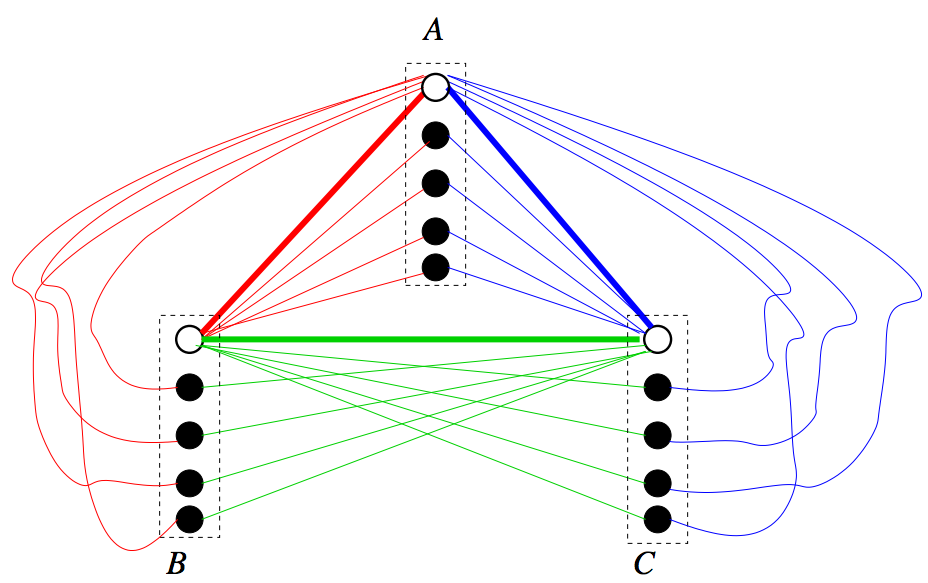
\includegraphics[scale=0.2]{triangle.png}
\end{center}
\caption{A counter-example which demonstrates why pair-wise plans for the triangle query are suboptimal. See \cite{ngo2014skew} for a thorough explanation.}
\end{figure}

First, rather than fix an order of relations to join, we instead fix some order of \emph{attributes}. Doing so enables us to ``look ahead'' and ensure that we don't unnecessarily materialize an intermediate relation that could prove to be wasteful later on in the computation. Without loss of generality, let our order $U = (A, B, C)$. We first compute candidates for attribute $A$, which we denote as $C_A$. To do this, we examine each relation with $A$ in its attribute set, and then compute the following: $C_A = \pi_A (R) \cap \pi_A (T)$. We can now guarantee that, for every possible triangle $(a_i, b_j, c_k)$ in the final output, $a_i \in C_A$ will always hold true. In other words, $C_A$ gives us the list of candidate values for attribute $A$ that may participate in the final output.

Next, we compute candidates for attribute $B$, which is next in our order $U$. We use the same approach as before, but we now incorporate our $C_A$ candidate values. For each $a_i \in C_A$, we evaluate $C_{AB} = \{a_i\} \times \big(\pi_B (\sigma_{A = a_i} R) \cap \pi_B (T)\big)$. Just as before, we maintain the invariant that every tuple $(a_i, b_j) \in C_{AB}$ is a candidate tuple for the final output.

Lastly, for attribute $C$, we iterate through each candidate $(a_i, b_j) \in C_{AB}$, and evaluate $C_{ABC} = \{a_i, b_j\} \times \big(\pi_C (\sigma_{B = b_j} S) \cap \pi_C (\sigma_{A = a_i} T)\big)$. The candidate set $C_{ABC}$ now equals our final output.

\begin{figure}[h]
\label{fig:walkthrough}
  \begin{minipage}[b]{0.55\linewidth}
  \centering
  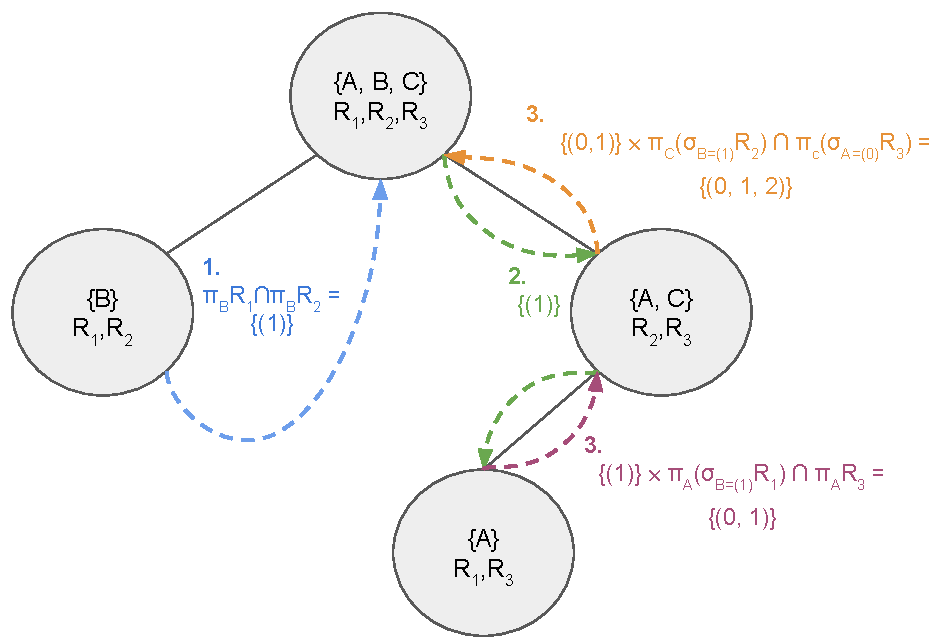
\includegraphics[scale=0.55]{walkthrough.pdf}
  \end{minipage}
  \begin{minipage}[b]{0.45\linewidth}
  \centering
  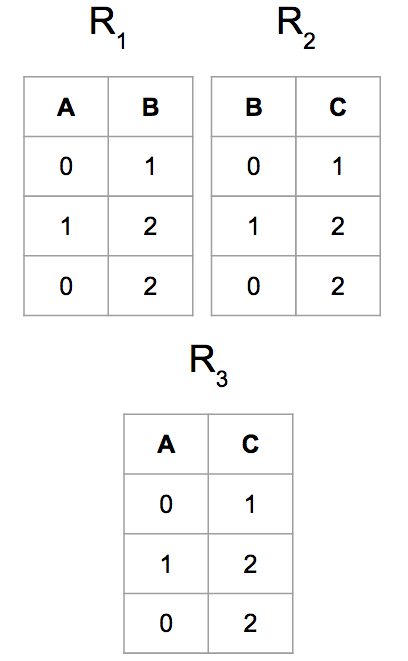
\includegraphics[scale=0.22]{table_walkthrough.png}
  \end{minipage}
\caption{A walkthrough of the NPRR algorithm on the triangle query. Here the attribute order $U = (B,A, C)$.}
\end{figure}

\section{Implementation}


\section{Results}

We now evaluate the performance of NPRR, PostgreSQL and an in-memory triangle counting baseline. We release all the source codes of the algorithms used in our evaluation in \url{https://github.com/fabuzaid21/nprr}.


\textbf{Datasets.} We used four large real-world datasets, which are from four different domains as shown in Table~\ref{datasets}. Facebook consists of 'circles' (or 'friends lists') from Facebook. Gnutella is a sequence of snapshots of the Gnutella peer-to-peer file sharing network from August 2002. Wikivote consists of votes deciding who is going to  be promoted as adminship. Condmat (Condense Matter Physics) collaboration network covers scientific collaborations between authors papers submitted to Condense Matter category. 


\begin{table}[!h]
\centering

\begin{tabular}{|l|l|l|}
\hline
Data & $|V|$ & $|E|$ \\
\hline
facebook & 4039 & 88234  \\
\hline
gnutella & 36682 & 88328 \\
\hline
wikivote & 7115 & 103689 \\
\hline
condmat & 23133 & 93479 \\
\hline
\end{tabular}
\caption{Datasets}
\label{datasets}
\end{table}



\textbf{Experimental settings.} We ran our experiments on a machine with a 2.4GHz Intel(R) Core(R) i5-4258U CPU and 8 GB DDR3-1,6000 RAM, running 64-bit MacOSX 10.11.2. NPRR was compiled with clang-700.1.81(Apple LLVM version 7.0.2). The optimization flag O2 option was enabled. PostgreSQL 9.4.5 was used during evaluation. 



\input{"postgres_integration.tex"}

\section{Future Work}

\section{Conclusion}


As many large scale data analytics engines emerge such as Spark and F1, queries are becoming more and more complex. However, the performance of evaluating a join query using a pair-wise manner could be highly suboptimal. In this paper, we studied a worst-case optimal join algorithm was established by Ngo, Porat, R$\acute{e}$ and Rudra. We implemented these ideas to see how they compare to the algorithms in a modern RDBMS and describe a detailed implementation and possible integration on PostgreSQL and Spark. Experiments on real world graphs verified that NPRR is able to achieve 2-6 times performance improvements over the state-of-the-art RDBMS.




\bibliographystyle{abbrv}
\bibliography{cite}

\appendix
\section{Native implementation}\label{native}

\begin{lstlisting}
#include <stdio.h>
#include <stdlib.h>
#include <sys/time.h>

#include<vector>
#include<map>

using namespace std;

vector<pair<int, int> > rel1;
map<int, vector<int> > rel2;
map<int, vector<int> > rel3;

double get_wall_time(){
    struct timeval time;
    if (gettimeofday(&time,NULL)){
        //  Handle error
        return 0;
    }
    return (double)time.tv_sec + (double)time.tv_usec * .000001;
}

int main(int argc, char **argv) {
  FILE *fin = fopen(argv[1], "r");

  double t1 = get_wall_time();
  
  while (true) {
    int a,b;
    int nRet = fscanf(fin, "%d %d", &a, &b);
    if (nRet != 2) {
      break;
    }


    rel1.push_back(make_pair(a,b));

    if (!rel2.count(a)) {
      vector<int> v;
      rel2[a] = v;
    }

    rel2[a].push_back(b);

    
    if (!rel3.count(a)) {
      vector<int> v;
      rel3[a] = v;
    }

    rel3[a].push_back(b);
  }

  double t2 = get_wall_time();

  int nTriangles = 0;

  for (auto x : rel1) {
    int a = x.first;
    int b = x.second;

    if (rel2.count(b)) {
      for (int c : rel2[b]) {
        if (rel3.count(a)) {
          for (int cp : rel3[a]) {
            if (c == cp) {
              nTriangles++;
            }
          }
        }
      }
    }
  }

  printf("%d\n", nTriangles);

  double t3 = get_wall_time();

  printf("Reading time: %f\n", t2-t1);
  printf("Computation time: %f\n", t3-t2);
  

  return 0;
}
	
\end{lstlisting}


\end{document}
